\chapter{Módulo firmware}

En este capítulo se especificarán todos los detalles relacionados con la programación que se ha llevado a cabo en la placa Node MCU ESP8266 \cite{nodemcuwikipedia}.

Esta placa permite al usuario que se programe tanto en LUA \cite{luawikipedia}, MicroPython \cite{micropython} o Arduino \cite{arduino}.

Para la realización de este proyecto se ha elegido el lenguaje de programación de Arduino ya que está basado en C y me siento más cómodo con este lenguaje en comparación con micropython. Además los códigos en C son algo más rápidos y podrían ocupar algo menos de memoria.

\section{Requisitos}

\subsection{Requisitos funcionales}

\begin{itemize}
	\item\textbf{RF1: } Introducir manualmente las credenciales de la conexión WiFi así como el tiempo que tardará en enviarse la información al servidor.
	\item\textbf{RF2: } Comprobar que el dispositivo está correctamente conectado a la red WiFi.
	\item\textbf{RF3: } Recoger la información de los sensores.
	\item\textbf{RF4: } Manejar la información obtenida para mostrar información util para el usuario.
	\item\textbf{RF5: } Mostrar dicha información al usuario mediante una pantalla.
	\item\textbf{RF6: } Enviar dicha información a un servidor para poder tener todos los datos almacenados.
\end{itemize}

\subsection{Requisitos no funcionales}

\begin{itemize}
	\item\textbf{RNF1: } La conexión WiFi del dispositivo ha de ser estable ya que si no los datos no podrían sen enviados al servidor.
	\item\textbf{RNF2: } La información que se muestra en la pantalla LCD se borrará antes de mostrar información nueva para evitar que la información se muestre en lugares de la pantalla inadecuados.
\end{itemize}

\section{Planificación}

\begin{itemize}
	\item\textbf{Fase 1: } Reunión con la persona interesada para concretar los detalles del proyecto que se quieren llevar a cabo.
	\begin{itemize}
		\item\textbf{Recopilar la información}  sobre los detalles que nos especifique la persona interesada.
		\item\textbf{Estudiar}  si es factible llevar a cabo las peticiones que se nos han hecho.
		\item Tener una \textbf{segunda reunión} para concretar las cosas que se pueden llevar a cabo y las que no.
	\end{itemize}
	\item\textbf{Fase 2: } Estudio para decidir en que lenguaje se va a llevar a cabo la programación y como se va proceder para enviar los datos al servidor.
	\begin{itemize}
		\item\textbf{Investigar}  que lenguaje de programación de los 3 (LUA, Micropython, Arduino) que permite el ESP8266 nos interesa más para llevar a cabo este proyecto.
		\item\textbf{Estudiar}  como interpretar los datos recogidos por el sensor para transformarlos en datos legibles por parte del usuario.
		\item\textbf{Estudiar}  cual es la mejor forma de mostrar la información en la pantalla LCD para mostrarla al usuario.
		\item\textbf{Estudiar}  cuál es la mejor forma de mandar los datos al servidor.
		\item\textbf{Estudiar}  cuales son las bibliotecas necesarias para realizar las labores citadas anteriormente.
	\end{itemize}
	\item\textbf{Fase 3: } Programación de los distintos módulos.
	\begin{itemize}
		\item\textbf{Programación}  del módulo de cálculo de irms (valor eficaz) \cite{valoreficaz}.
		\item\textbf{Programación}  del módulo para mostrar la información en la pantalla LCD.
		\item\textbf{Programación} del módulo para enviar la información al servidor.
	\end{itemize}
	\item\textbf{Fase 4: } Pruebas.
	\begin{itemize}
		\item\textbf{Pruebas}  de los distintos módulos que se han programado.
	\end{itemize}
	
\end{itemize}

\section{Arquitectura del firmware}

En este apartado se va a detallar el desarrollo de los distintos módulos que han sido necesarios para la elaboración de este proyecto.

\subsection{Módulo de lectura de sensor y cálculo de irms y potencia}

\begin{itemize}
\item\textbf{Lectura del sensor:}  La lectura de los valores del sensor se realizarán mediante el conversor analógico digital ADS1115. Para ello haremos uso de la biblioteca proporcionada por Adafruit en concreto la Adafruit\textunderscore ADS1x15 \cite{adafruitbib} válida tanto para ls versión 1015 de 12 bits como para la versión 1115 de 16 bits.

Esta biblioteca nos permite leer los valores de los pines desde el A0 hasta el A3 bien sea de forma única \textit{singleended} como calculando la diferencia entre dos pines \textit{differential} a parte de una tercera forma \textit{comparator}. En nuestro caso utilizaremos el modo que calcula la diferencia entre dos pines, es decir la función :

\begin{listing}[style=consola, numbers=none]
	int16_t readADC_Differential_0_1();
\end{listing} 

Esta biblioteca la podemos encontrar en el repositorio de GitHub de Adafruit \cite{adafruitbib}.

\item\textbf{Cálculo de irms y potencia:} Para este proyecto se van a calcular el irms o valor eficaz \cite{valoreficaz} y a partir de ahí la potencia real.

Tras ver los resultados obtenidos por el sensor tal cuál los leemos gracias a la función de la biblioteca de Adafruit mencionada anteriormente. Estamos midiendo corriente alterna, la cuál está cambiando constantemente, por lo tanto tendremos valores con una polaridad negativa y otros con polaridad positiva. Dependiendo del tipo de onda obtenida la fómula que hay que aplicar para calcular el irms cambiará. En la gráfica (\ref{fig:graficasensorraw}) podemos ver que los valores que capta el sensor son tanto positivos como negativos obteniendo esta onda. Por lo tanto no nos interesa obtener ni la media de todos estos valores obtenidos por el sensor ni el valor pico de la onda lo que nos interesa calcular es el valor eficaz. En nuestro caso particular según la bibliografía \cite{mediacuadraticawiki} para calcular el irms de una onda sinosoidal generada al medir corriente alterna la solución es simplemente calcular la media cuadrática aplicando la fórmula de esta media \cite{mediacuadraticawiki} $ \sqrt{\frac{x^2_{1} + x^2_{1} + ... + x^2_{n}}{N}}$.


\begin{figure}[H]
	\centering
	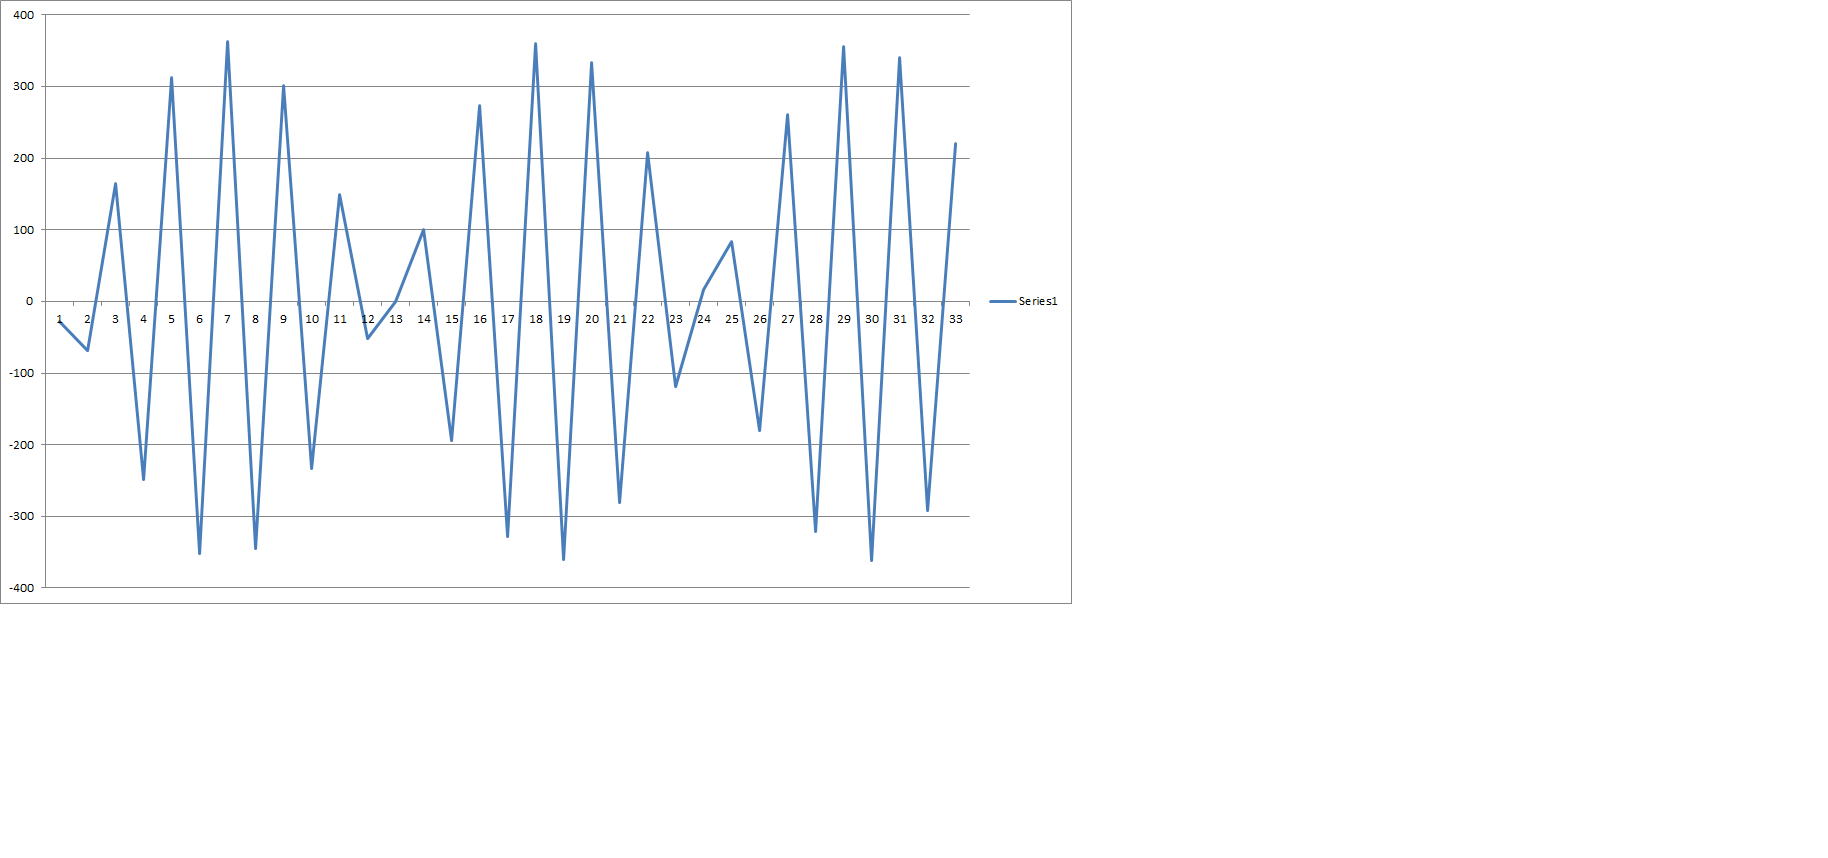
\includegraphics[scale=0.5]{imagenes/datossensorraw.png}
	\caption{Representación datos obtenidos del sensor.}
	\label{fig:graficasensorraw}
\end{figure}

Pero antes de realizar este cálculo tendremos que calcular el offset mediante un filtro de paso bajo software al tratarse de un filtro paso bajo el offset corresponde a los valores más altos de la onda y tendremos que restar este valor de offset, de esta forma conseguimos dejar la onda lo más centrada posible atenuando los valores altos y dejando pasar los más bajos \cite{pasobajowikipedia} . En nuestro caso el sistema se está alimentando con 3.3V por lo tanto el offset que se le resta a la muestra es el equivalente a una corriente de 1,65V.

Lo que conseguimos restándole este offset al valor obtenido mediante el sensor es eliminar ese voltaje que tiene de por si el sistema aunque no se esté midiendo nada es decir cuando esta en reposo. De todas formas el sistema se calibrará gracias a la variable ICAL ya que dependiendo del sistema que montemos la calibración variará.

Una vez calculado el irms (A) podremos calcular la potencia real (W) del aparato que estemos midiendo gracias a la ley de Watt y la ley de Ohm obteniendo la fórmula $ P(W) = (irms(A) \cdot V(V))$ 


\begin{figure}[H]
	\centering
	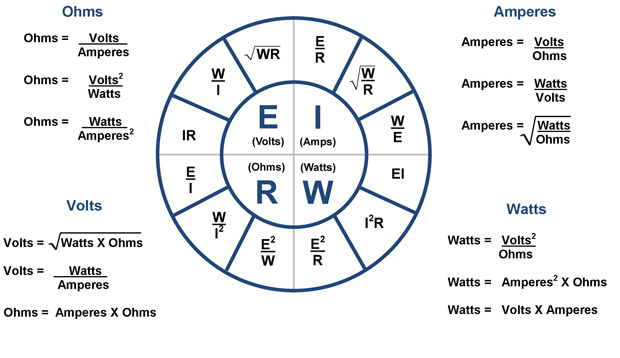
\includegraphics[scale=0.7]{imagenes/equation.jpg}
	\caption[Ley de Ohm y Watt.]{Ley de Ohm y Watt. Fuente \cite{calculadoraohm}.}
	\label{fig:formulaondas}
\end{figure}


\end{itemize}

\subsection{Módulo para mostrar información en la pantalla LCD}

Para mostrar información en una pantalla LCD no existen bibliotecas exclusivas diseñadas para el ESP8266 pero esta biblioteca \textit{LiquidCrystal\textunderscore I2C.h} diseñada para Arduino \cite{lcdgithub} nos permitirá mostrar la información que queramos sin ningún tipo de problema. Al estar compartiendo la conexión I2C con el conversor analógico digital tendremos que especificar en la creación del objeto la dirección de memoria de la pantalla LCD. 

Una vez creado el objeto tan solo tendremos que llamar a la función creada para mostrar la información deseada la cuál se le pasará a la función como argumentos:

\begin{listing}[style=consola, numbers=none]
	void imprimirLcd(double irms, double potencia){
		lcd.clear();
		lcd.print("irms: ");lcd.print(irms);lcd.print("A");
		lcd.setCursor(0,1);
		lcd.print("Potencia: ");lcd.print(potencia);lcd.print("W");
	}
\end{listing} 



\subsection{Módulo envío de información al servidor}

Para el envío de la información se ha decidido enviarla mediante HTTP (Hypertext Transfer Protocol), se trata de un protocolo de comunicación en red que hace posible la comunicación entre un cliente y un servidor mediante peticiones por parte del cliente y respuestas por parte del servidor \cite{httpinfo}. Para este proyecto vamos a utilizar el método de petición POST mediante el cuál seremos capaces de enviar la información que deseemos especificando la URL del servidor donde queramos enviar dicha información, cuado esa información sea recibida por el servidor se enviará una respuesta al cliente que generó la petición POST.  Gracias a la biblioteca \textit{ESP8266HTTPClient.h} \cite{httpclientgithub} una biblioteca para dispositivos IoT es posible realizar (entre otros métodos implementados en esta biblioteca) una petición POST de una manera muy sencilla en la placa ESP8266 en concreto gracias a la función:

\begin{listing}[style=consola, numbers=none]
	int POST(String payload);
\end{listing} 

A la hora de escoger en que formato enviar la información al servidor se ha escogido JSON (JavaScript Object Notation) que no es más que un formato para para realizar intercambio de datos. Haciendo uso de la biblioteca \textit{ArduinoJson.h} \cite{jsongithub} con la que podremos codificar arrays o incluso añadir valores al objeto creado directamente. 

Todo esto se realizará llamando a la función que se ha creado para hacer el código más legible. Pero la parte correspondiente únicamente a la codificación del JSON es la siguiente 

\begin{listing}[style=consola, numbers=none]
	StaticJsonBuffer<300> JSONbuffer;   //Declarar JSON buffer
	JsonObject& JSONencoder = JSONbuffer.createObject();
	
	JSONencoder["sensorType"] = "Power";
	Serial.println("irms dentro de mandarjson: ");Serial.println(irms);
	JsonArray& values = JSONencoder.createNestedArray("values"); //JSON array
	values.add(irms); //Aniadir valor al array
	values.add(potencia); //Aniadir valor al array
	
	JsonArray& valuesInfo = JSONencoder.createNestedArray("valuesInfo"); //JSON array
	valuesInfo.add("irmsnuevo"); //Aniadir valor al array
	valuesInfo.add("potencianueva"); //Aniadir valor al array
	
	char JSONmessageBuffer[300];
	JSONencoder.prettyPrintTo(JSONmessageBuffer, sizeof(JSONmessageBuffer));
	Serial.println(JSONmessageBuffer);


\end{listing} 



